\documentclass{beamer}
\usetheme{CambridgeUS}
%\usebeamercolor{lily}
%\useoutertheme{miniframes}
\useoutertheme{infolines}
%\useoutertheme{shadow}
\usefonttheme{serif}
\usepackage{graphicx}
\usepackage{setspace}
\usepackage{tabularx}
\usepackage{tikzsymbols}
\usepackage{tikz}
\usepackage{spot}
\usepackage[italian]{babel}
\usepackage{tabularx}
\usepackage[absolute,overlay]{textpos}
\usepackage{booktabs}
\usepackage{fancyvrb}
\usepackage{xcolor}
\usepackage{multicol}
\usepackage{multirow}


\newcommand\Factor{1.2}


%\setbeamertemplate{footline}[page number]
\setbeamerfont{subtitle}{size=\large, series=\bfseries}
\definecolor{template}{RGB}{54, 114, 89}
\definecolor{background}{RGB}{250, 250, 250}
\setbeamercolor{frametitle}{fg=template, bg=white}
\setbeamercolor{section in head/foot}{bg=template, fg=template!20}
\setbeamercolor{subsection in head/foot}{bg=template!20, fg=template}
\setbeamercolor{author in head/foot}{bg=template, fg=template!20}
\setbeamercolor{date in head/foot}{bg=template, fg=white}
\setbeamercolor{page number in head/foot}{bg=template, fg=white}
\setbeamercolor{title in head/foot}{fg=template}
\setbeamercolor*{item}{fg=template}
\setbeamertemplate{frametitle}{\color{template}\bfseries\scshape\insertframetitle\par\hrulefill}
\setbeamercolor{title}{fg=template}
\definecolor{highlight}{RGB}{54, 114, 89}
\definecolor{back}{RGB}{247, 251, 255}
\definecolor{map}{RGB}{111, 172, 232}
\definecolor{childmap}{RGB}{161, 200, 240}
\definecolor{nodemap}{RGB}{141, 170, 199}
\definecolor{rasch}{rgb}{0.0, 0.33, 0.71}
\definecolor{log}{rgb}{0.0, 0.65, 0.58}
\definecolor{diff}{RGB}{33, 113, 181}
\definecolor{single}{RGB}{106, 81, 163}
\definecolor{comp}{RGB}{35, 99, 70}
\definecolor{inc}{RGB}{191, 13, 43}
\definecolor{highlight}{rgb}{0.45, 0.31, 0.59}
\definecolor{section}{RGB}{51,51,179}
\definecolor{typical}{RGB}{8, 69, 148}
\definecolor{model}{RGB}{74, 20, 134}
\definecolor{orangered2}{RGB}{238,64,0}
\definecolor{royalblue3}{RGB}{58,95,205}
\definecolor{springgreen}{RGB}{0,205,102}
\definecolor{magenta}{RGB}{255,0,255}

  \tikzset{
	invisible/.style={opacity=0},
	visible on/.style={alt={#1{}{invisible}}},
	alt/.code args={<#1>#2#3}{%
		\alt<#1>{\pgfkeysalso{#2}}{\pgfkeysalso{#3}} % \pgfkeysalso doesn't change the path
	},
	every overlay node/.style={
		%draw=black,fill=white,rounded corners,
		anchor=north west, inner sep=0pt,
	},
}

\def\tikzoverlay{%
	\tikz[remember picture, overlay]\node[every overlay node]
}%


\AtBeginSection[]
{
	\begin{frame}
		\tableofcontents[currentsection,currentsubsection]
	\end{frame}
}  



%\title[Implicit assessment]{Implicit assessment in psychology: \\ How to work with the IAT}
\title[Experiment set up]{Misurazione Implicita in Psicologia: \\ Programmare gli esperimenti in Inquisit}
\date[PSQT, 2023]{Master di II Livello \\ Psicologia quantitativa: Misurazione, valutazione e analisi di variabili psicosociali }
\institute[]{18 luglio 2024, Padova}
\author[Ottavia M. Epifania]{\texorpdfstring{Ottavia M. Epifania, Ph.D.\newline\url{ottavia.epifania@unipd.it}}{Author}}

\begin{document}
	\tikzstyle{every picture}+=[remember picture]
	


\begin{frame}[plain]
    \maketitle
\end{frame}

\section*{Questo corso}

\begin{frame}
Mattino: 
\begin{itemize}
	\item Programmazione degli esperimenti in Inquisit
\end{itemize}

Pomeriggio:
\begin{itemize}
	\item Calcolo degli indici: 
	\begin{itemize}
		\item in \texttt{R}
		\item App online
	\end{itemize}
\end{itemize}

A casa: 
\begin{itemize}
	\item Creare 4 condizioni sperimentali a seconda dell'ordine di presentazione delle domande esplicite e delle condizioni associative dello IAT
	\item Calcolo degli indici e loro correlazione!
\end{itemize}

\end{frame}



\section{Cosa ci serve}

\begin{frame}
	
	\begin{itemize}
			\item Download \href{https://www.millisecond.com/download/}{
\includegraphics[width=0.10\linewidth]{inquisit.png}} e seguire le istruzioni \textcolor{red}{!!! la demo è valida solo per un mese!!}
			\item Download \href{https://www.millisecond.com/download/library/iat/ageiat}{\textcolor{blue}{AGE IAT}} da Inquisit test library
		\item A \href{https://www.millisecond.com/download/library}{\textcolor{blue}{questo indirizzo}} trovate tutti gli esperimenti che sono stati implementati fino ad ora in Inquisit  
		\item A \href{https://www.millisecond.com/support/docs/current/html/main.htm}{\textcolor{blue}{questo indirizzo}} trovate una guida completa sull'utilizzo di Inquisit
	\end{itemize}
\end{frame}

\begin{frame}
	Aprite il file 
	
	\vspace{3mm}
	Fate ``correre'' l'esperimento e compilatelo 
	
	\vspace{3mm}
	Una volta terminato, caricate il file \texttt{.dat} (dategli un nome nuovo e unico) \href{https://drive.google.com/drive/folders/1qdGvU1hlttucNOU2Sy_1EVKazj8QnBlu?usp=sharing}{\textcolor{blue}{qui}} 
	
	\begin{exampleblock}{Esempio}
		
		\texttt{dati-Mario-Rossi.dat}
	\end{exampleblock}
	
	\vspace{3mm}
	Vi è piaciuto l'esperimento? Avreste fatto qualcosa di diverso? Avreste aggiunto o tolto qualcosa? 
	

\end{frame}

\section{Il file Inquisit}

\subsection*{Default}

\begin{frame}
	\begin{enumerate}
		\item User manual (Potete tenerlo o meno)
		\item Pagina di benvenuto
		\item Etichette e stimoli
		\item Pagine di istruzione \& summary dei risultati
		\item Preparare il materiale
		\item Preparare i ``blocchi'' dell'esperimento
		\item L'esperimento vero e proprio
	\end{enumerate}
\end{frame}

\begin{frame}[fragile]{Gli elementi di default}
	Non si toccano!
	
	\begin{Verbatim}
<defaults>
/ fontstyle = ("Arial", 3.5%, false, false, false, 
    false, 5, 1)
/ screencolor = black
/ txbgcolor = black
/ txcolor = white
/ minimumversion = "6.5.2.0"
/ canvasaspectratio = (4, 3) %è la dimensione del 
	% contenitore degli stimoli
</defaults>
	\end{Verbatim}
\end{frame}

\subsection*{Welcome}


\begin{frame}[fragile]{Pagina di benvenuto}
	
	\begin{columns}
	\begin{column}{.50\linewidth}
		\begin{small}
\begin{verbatim}
<htmlpage iatintro>
/ file = "intro_pictureiat.htm"
</htmlpage>
			\end{verbatim}
		\end{small}
	\end{column}

	\begin{column}{.50\linewidth}
		\centering
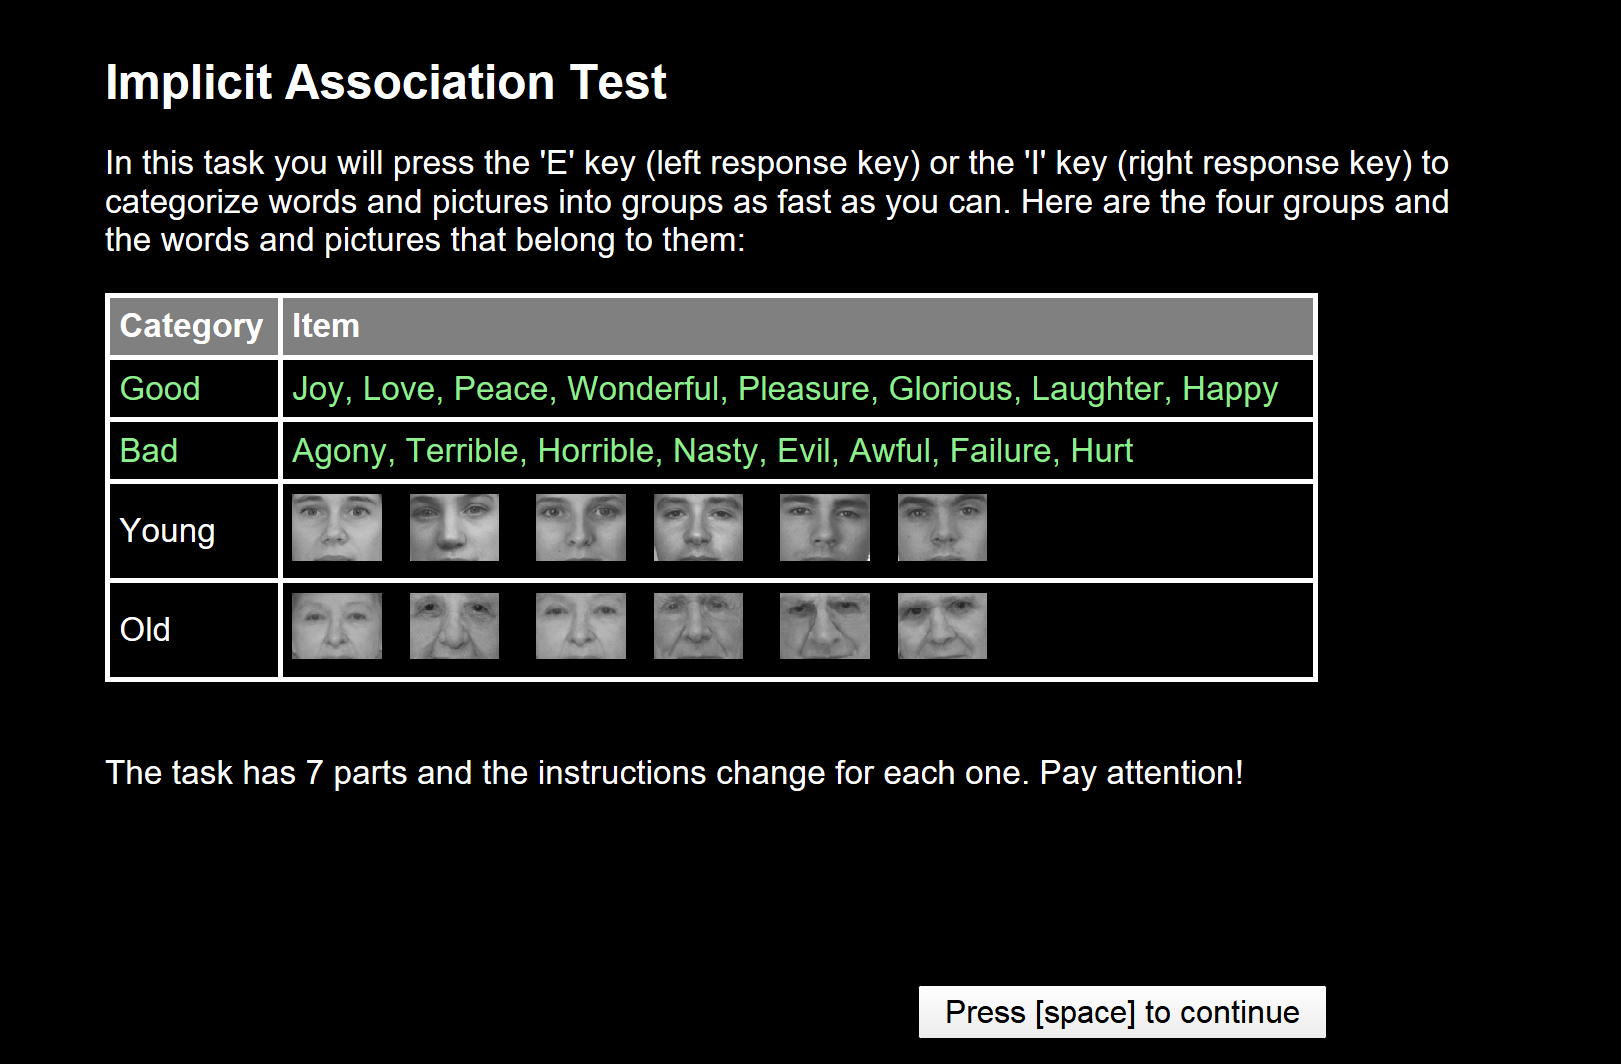
\includegraphics[width=\linewidth]{iatIntro.png}
   \end{column}
	\end{columns}
	
\end{frame}

\begin{frame}[fragile]
	 \texttt{intro\_pictureiat.htm} Si apre con il blocco note 
	
\begin{footnotesize}
		\begin{verbatim}
		<!DOCTYPE html>
		<html>
		<head>
		<meta charset="UTF-8">
		<meta name="robots" content="noindex, nofollow"/> 
		<title>iat intro</title>
		<style>
		.center {
			text-align: center;
		}
		.left {	
			text-align: left;
		}
		[.....]
	\end{verbatim}
\end{footnotesize}

Può essere modificato e salvato (ad esempio, per mettere le istruzioni in italiano)
\end{frame}

\subsection*{La logica}

\begin{frame}[fragile]{Logica di Inquisit}
	\begin{enumerate}
		\item Definire gli oggetti da mostrare (siano immagini, istruzioni, parole) con \texttt{<item></item>}
		\item Impostare il loro aspetto (con \texttt{<text></text>} se stimoli parole o con \texttt{<picture></picture>} se stimoli immagine)
		\item Impostare il loro comportamento con \texttt{<trial></trial>}
		\item Definire i blocchi che verranno usati nell'esperimento con \texttt{<block></block>}
		\item Impostare l'esperimento vero e proprio con \texttt{<expt></expt>}
	\end{enumerate}
\end{frame}

\subsection*{Etichette e stimoli}
%\frame{\tableofcontents[currentsection,currentsubsection]} 

\begin{frame}[fragile]
	Definire ``Attribute A'' (in questo caso, ``\textcolor{green}{Good}'')
	
	\begin{columns}
		\begin{column}[T]{.50\linewidth}
			\begin{small}
					\begin{Verbatim}[commandchars=\\\{\}]
<item \textcolor{red}{attributeAlabel}>
/1 = "Good"
</item>
					
<item \textcolor{red}{attributeA}>
/1 = "Joy"
/2 = "Love"
/3 = "Peace"
/4 = "Wonderful"
/5 = "Pleasure"
/6 = "Glorious"
/7 = "Laughter"
/8 = "Happy"
</item>
				\end{Verbatim}
			\end{small}
		\end{column}
	
		\begin{column}[T]{.50\linewidth}
			\vspace{5mm}
		Definisce l'etichetta che verrà mostrata sullo schermo per la dimensione valutativa ``A'' (i.e., ``Good'')
		
		\vspace{10mm}
		
		Elenco di tutte le parole che appartengono a ``Good''
		
		Per aggiungere ulteriori parole: \\ \texttt{/9 = ``Bello''  \\  /10 = ``Carino''}
	\end{column}
	\end{columns}



\end{frame}

\begin{frame}[fragile]
	Si fa la stessa cosa per gli stimoli target. 
	Si usa la stessa sintassi, ma questa volta si importano le immagini stimolo del ``Target A'' (in questo caso ``Young'' ). Le immagini devono essere nella stessa cartella.
	
	\begin{columns}
		\begin{column}[T]{.40\linewidth}
			\begin{small}
			\begin{Verbatim}[commandchars=\\\{\}]
<item \textcolor{red}{targetAlabel}>
/1 = "Young"
</item>
				
<item \textcolor{red}{targetA}>
/1 = "yf1.jpg"
/2 = "yf4.jpg"
/3 = "yf5.jpg"
/4 = "ym2.jpg"
/5 = "ym3.jpg"
/6 = "ym5.jpg"
</item>
			\end{Verbatim}
			\end{small}
		\end{column}
		
		\begin{column}[T]{.60\linewidth}
			\vspace{5mm}
				Definisce l'etichetta che verrà mostrata sullo schermo per la categoria target ``Young'' (i.e., ``Young'')
			
			\vspace{7mm}
			
			Elenco di tutte le immagini che appartengono a ``Young''
			
			Per aggiungere ulteriori parole: \\ \texttt{/7 = ``yg6.jpg''  \\  /8 = ``ym7.jpg''}
		\end{column}
	\end{columns}
	
\end{frame}

\begin{frame}
\begin{center}
	
\includegraphics[width=.20\linewidth]{work.png}
\end{center}
\begin{itemize}
	\item Traducete in italiano i nomi delle categorie che appaiono nella Welcome page (il file \texttt{intro\_pictureiat.htm})
	
	\item Traducete in italiano i nomi delle categorie nel file Inquisit
	
	\item Aggiungete una parola per ognuna delle due categorie attributo
	
	\item Aggiungete un'immagine per ognuna delle categorie target (cercatele su Google!)
\end{itemize}
\end{frame}

\subsection*{Pagine di istruzione}

\begin{frame}[fragile]{Simboli di navigazione}
	
	\begin{figure}
		\centering
		
\includegraphics[width=0.3\linewidth]{navigation}
	\end{figure}
	
		\begin{verbatim}
			<instruct>
			/ navigationbuttonfontstyle = 
			("Arial", 3%, false, false, false, false, 5, 1)
			</instruct>
		\end{verbatim}
	
	Definisce l'aspetto del bottone di navigazione. 
	\end{frame}

\begin{frame}[fragile]{Cambiare il font}
	
	\begin{verbatim}
		("font-name", height, bold, italic, underline, strikeout, 
		quality, set)
	\end{verbatim}
	
	font-name: e.g., ``Arial'', ``Tahoma'', ``Courier New''
	
	quality: qualità del font, 1-5
	
	set: set dei caratteri (e.g., latin, greek. Se si utilizza 1, come in questo caso, viene preso il default del computer)
\end{frame}

\begin{frame}[fragile]{Le istruzioni}
	
	\begin{Verbatim}[commandchars=\\\{\}]
<item \textcolor{red}{instructions}>
/ 1 = "Put your left[...]."
	
/ 2 = "Put your left finger [...]"
	
/ 3 = "Press the left 'E' "
	
[...]
</item>
\end{Verbatim}

\vspace{2mm}
Le istruzioni vengono definite come una lista di item (vedremo anche un'altra opzione per creare le istruzioni)


\end{frame}

\begin{frame}[fragile]
	\begin{Verbatim}
'<%item.attributeAlabel.item(1)%>' 
	\end{Verbatim}

Non dovete scrivere voi a mano i nomi delle etichette delle categorie attributo, lo fa Inquisit per voi

\begin{verbatim}
	'<%expressions.leftTarget%>'
\end{verbatim}

Nel testo viene messa l'etichetta della categoria disposta sulla sinistra dello schermo. Viene usato l'argomento \texttt{expressions} perché la categoria che viene mostrata sul lato sinistro dello schermo dipende dalla condizione associativa dello IAT.

\end{frame}


%\begin{frame}[fragile]
%\begin{figure}
%	\centering
%	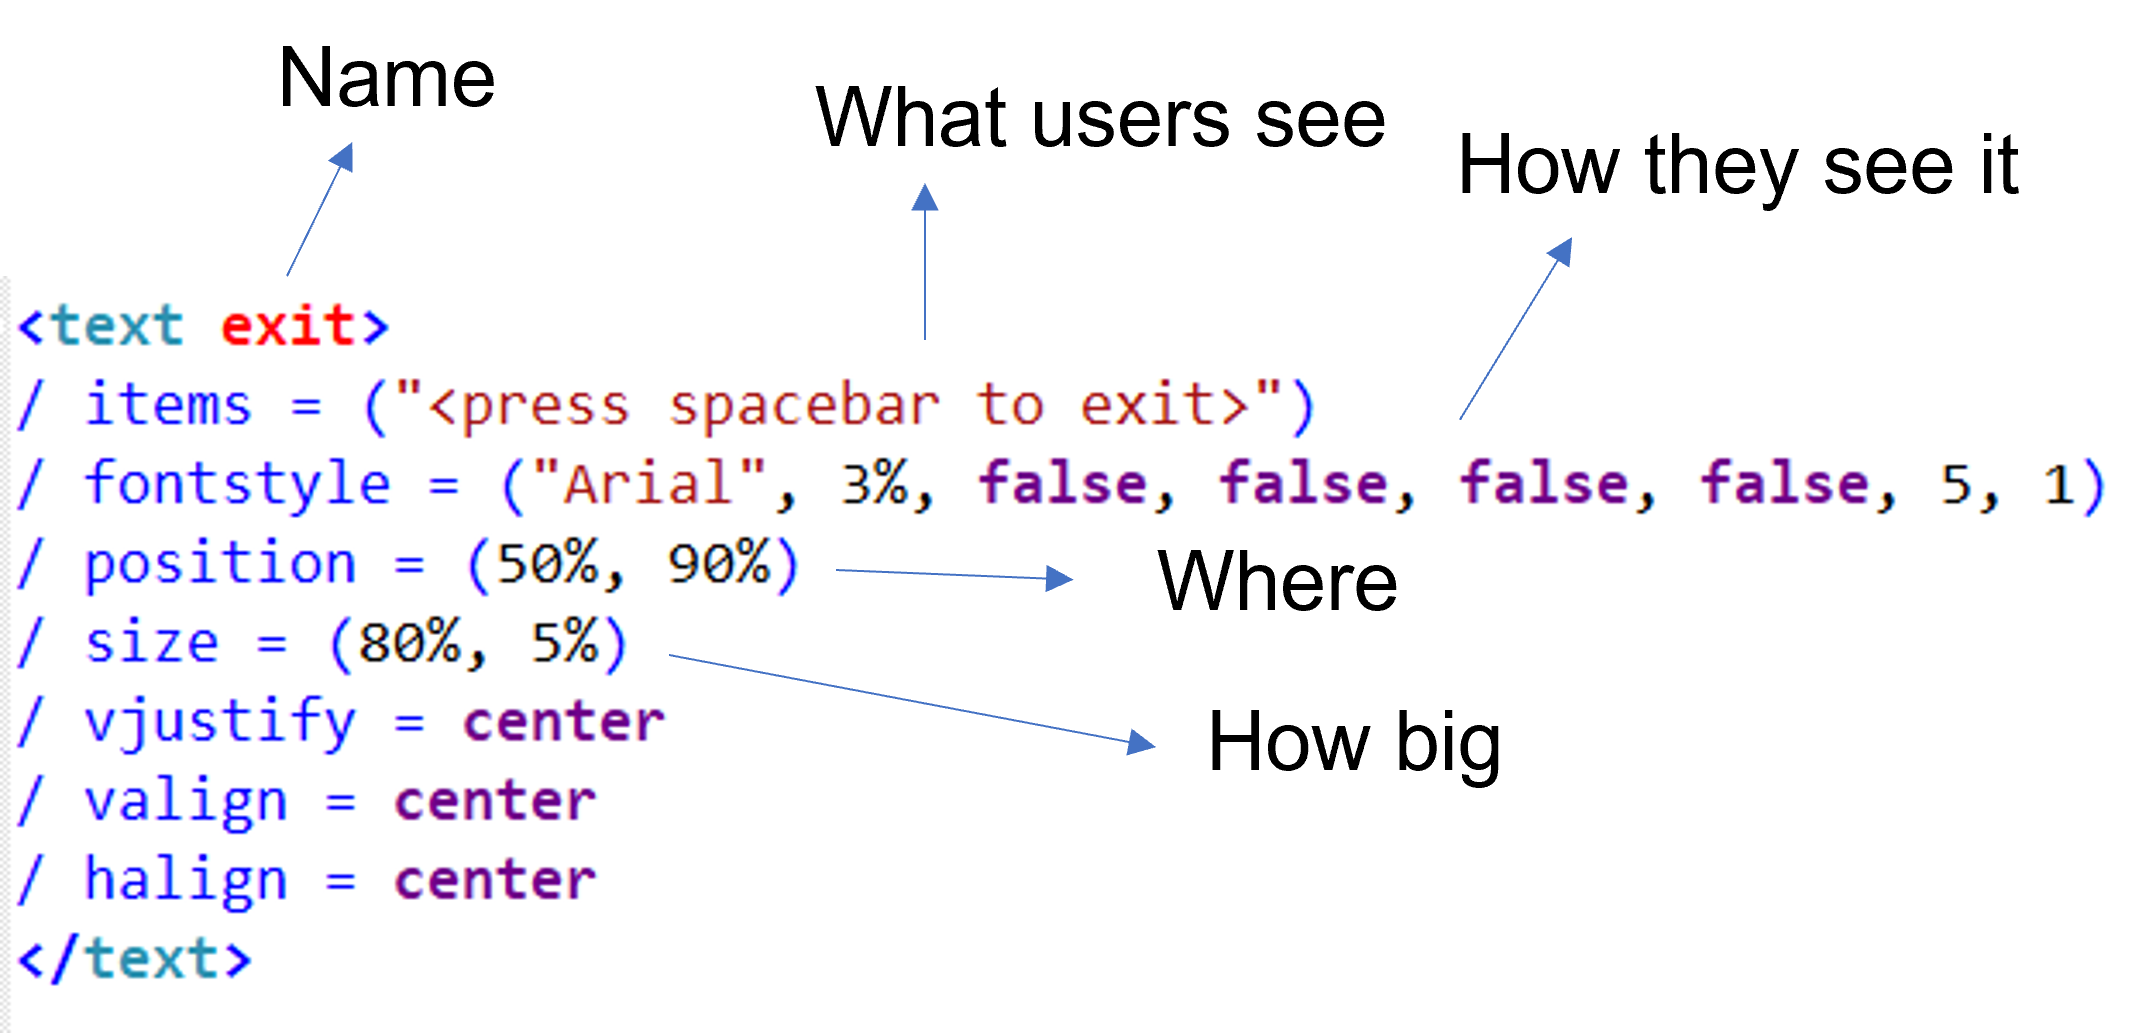
\includegraphics[width=.80\linewidth]{textThank.png}
%\end{figure}
%
%\vspace{3mm}
%No actual behavior has been defined yet
%\end{frame}

\subsection*{Impostare il materiale dell'esperimento}

\begin{frame}[fragile]{Definire l'aspetto degli elementi}

Sono stati solo definiti gli oggetti che verranno usati per l'esperimento.

Per definire l'aspetto degli oggetti ci sono delle funzioni apposite: 

\vspace{3mm}
\begin{columns}
\begin{column}{.50\linewidth}
	Per gli oggetti ``testo'':
	\begin{Verbatim}[commandchars=\\\{\}]
<text  \textcolor{red}{etichetta}>
/ items = \textcolor{red}{etichettaItem}
[...]
</text>
	\end{Verbatim}
\end{column}
\begin{column}{.50\linewidth}
	Per gli oggetti immagine:
		\begin{Verbatim}[commandchars=\\\{\}]
<picture \textcolor{red}{etichetta}>
/ items = \textcolor{red}{etichettaItem}
[...]
</picture>		
	\end{Verbatim}
\end{column}
\end{columns}
\end{frame}

\begin{frame}[fragile]{Esempio oggetti testo}
	
	\begin{small}
	\begin{Verbatim}[commandchars=\\\{\}]
<text \textcolor{red}{instructions}>
/ items = \textcolor{red}{instructions} % prendiamo <item \textcolor{red}{instructions}>
/ position = (10%, 25%)
/ halign = left
/ valign = top
/ hjustify = left
/ vjustify = center
/ size = (80%, 50%)
/ select = values.instructionIndex % 
</text>
\end{Verbatim}
	\end{small}

\texttt{/ select = values.instructionIndex} contatore per vedere la pagina corretta di istruzioni

\end{frame}


\begin{frame}[fragile]
	Stessa cosa con gli stimoli attributo:
	\vspace{3mm}
	\begin{Verbatim}[commandchars=\\\{\}]
<text \textcolor{red}{attributeA}>
/ items = \textcolor{red}{attributeA}
/ fontstyle = ("Arial", 5%)
/ txcolor = green
</text>
	\end{Verbatim}

		\begin{Verbatim}[commandchars=\\\{\}]
<text \textcolor{red}{attributeB}>
/ items = \textcolor{red}{attributeB}
/ fontstyle = ("Arial", 5%)
/ txcolor = green
</text>
	\end{Verbatim}
	
\end{frame}

\begin{frame}[fragile]{Esempio oggetti immagine}
	
	\begin{columns}
		\begin{column}{.50\linewidth}
Immagini della categoria target A: 
\begin{Verbatim}[commandchars=\\\{\}]
<picture \textcolor{red}{targetA}>
/ items = \textcolor{red}{targetA}
/ size = (20%, 20%)
</picture>
		\end{Verbatim}
		\end{column}
\begin{column}{.50\linewidth}
Immagini della categoria target B: 
\begin{Verbatim}[commandchars=\\\{\}]
<picture \textcolor{red}{targetB}>
/ items = \textcolor{red}{targetB}
/ size = (20%, 20%)
</picture>
		\end{Verbatim}
	\end{column}
	\end{columns}
\end{frame}

\begin{frame}[fragile]{Definire il comportamento degli oggetti}
\begin{small}
	\begin{Verbatim}[commandchars=\\\{\}]
<trial \textcolor{red}{etichettaTrial}>
/ validresponse = ("elenco", "risposte", "valide")
/ correctresponse = ("risposta corretta")
/ stimulusframes = [\textcolor{red}{1 = etichettaItem}, \textcolor{blue}{altre cose}]
/ posttrialpause = parameters.ISI
</trial>
	\end{Verbatim}
\end{small}
 

\texttt{\textcolor{red}{1 = etichettaItem}}: Gli stimoli che vengono inclusi

\texttt{\textcolor{blue}{altre cose}}: Altri elementi che sono presenti nel trial ma che non sono propriamente stimoli 

\end{frame}

\begin{frame}[fragile]{I trial di istruzione}
	\begin{small}
	
	\begin{Verbatim}[commandchars=\\\{\}]
<trial instructions>
/ ontrialbegin = [
values.progresswidth += 10; %riempimento barra avanzamento 
values.instructionIndex += 1; %contatore delle pagine di istr.
/ stimulustimes = [1=\textcolor{red}{instructions}, \textcolor{blue}{spacebar, progressbar}, 
\textcolor{blue}{progressbar_fill}]
/ correctresponse = (" ")
/ errormessage = false
/ recorddata = false
/ showmousecursor = true
</trial>
	\end{Verbatim}

	\end{small}


\end{frame}



\begin{frame}[fragile]{	Gli stimoli attributo}
	\vspace{3mm}
\begin{Verbatim}[commandchars=\\\{\}]
<trial attributeA>
/ validresponse = ("E", "I")
/ correctresponse = ("E")
/ stimulusframes = [1 = \textcolor{red}{attributeA}, \textcolor{blue}{errorReminder}]
/ posttrialpause = parameters.ISI
</trial>
	\end{Verbatim}
	\vspace{3mm}
\begin{Verbatim}[commandchars=\\\{\}]
<trial attributeB>
/ validresponse = ("E", "I")
/ correctresponse = ("I")
/ stimulusframes = [1 = \textcolor{red}{attributeB}, \textcolor{blue}{errorReminder}]
/ posttrialpause = parameters.ISI
</trial>
\end{Verbatim}
\end{frame}

\begin{frame}[fragile]{Gli stimoli immagine}

		\begin{Verbatim}[commandchars=\\\{\}]
<trial \textcolor{red}{targetAleft}>
/ validresponse = ("E", "I")
/ correctresponse = ("\textcolor{red}{E}")
/ stimulusframes = [1 = \textcolor{red}{targetA}, \textcolor{blue}{errorReminder}]
/ posttrialpause = parameters.ISI
</trial>
		\end{Verbatim}
Ma anche:
	\begin{Verbatim}[commandchars=\\\{\}]
<trial \textcolor{red}{targetAright}>
/ validresponse = ("E", "I")
/ correctresponse = ("\textcolor{red}{I}")
/ stimulusframes = [1 = targetA, errorReminder]
/ posttrialpause = parameters.ISI
</trial>
	\end{Verbatim}

\end{frame}

\begin{frame}
	\begin{center}
		
\includegraphics[width=.20\linewidth]{work.png}
	\end{center}
	\begin{itemize}
		\item Cambiate la dimensione degli stimoli immagine (leggermente più piccoli)
		
		\item Cambiate la dimensione degli stimoli parole (leggermente più piccoli)
		
		\item Cambiate il font degli stimoli parola e delle etichette (e.g., \texttt{Tahoma}, \texttt{Courier New})
		
		\item Cambiate i tasti di risposta: 
		\begin{itemize}
			\item stimoli categoria di sinistra: E $\rightarrow$ W
			\item stimoli categoria di sinistra: I $\rightarrow$ O
		\end{itemize}
	\end{itemize}
\end{frame}


\subsection*{I blocchi sperimentali}

\begin{frame}[fragile]{Blocchi di pratica ``pura''}
		\begin{small}
		\begin{Verbatim}[commandchars=\\\{\}]
<block \textcolor{red}{attributepractice}>
/ bgstim = (\textcolor{red}{attributeAleft}, \textcolor{red}{attributeBright})
/ trials = [
1=\textcolor{red}{instructions};
2-21 = random(\textcolor{blue}{attributeA}, \textcolor{blue}{attributeB});
]
/ errormessage = true(error,200)
/ responsemode = correct
</block>			
		\end{Verbatim}

%	\begin{figure}
%		\centering
%		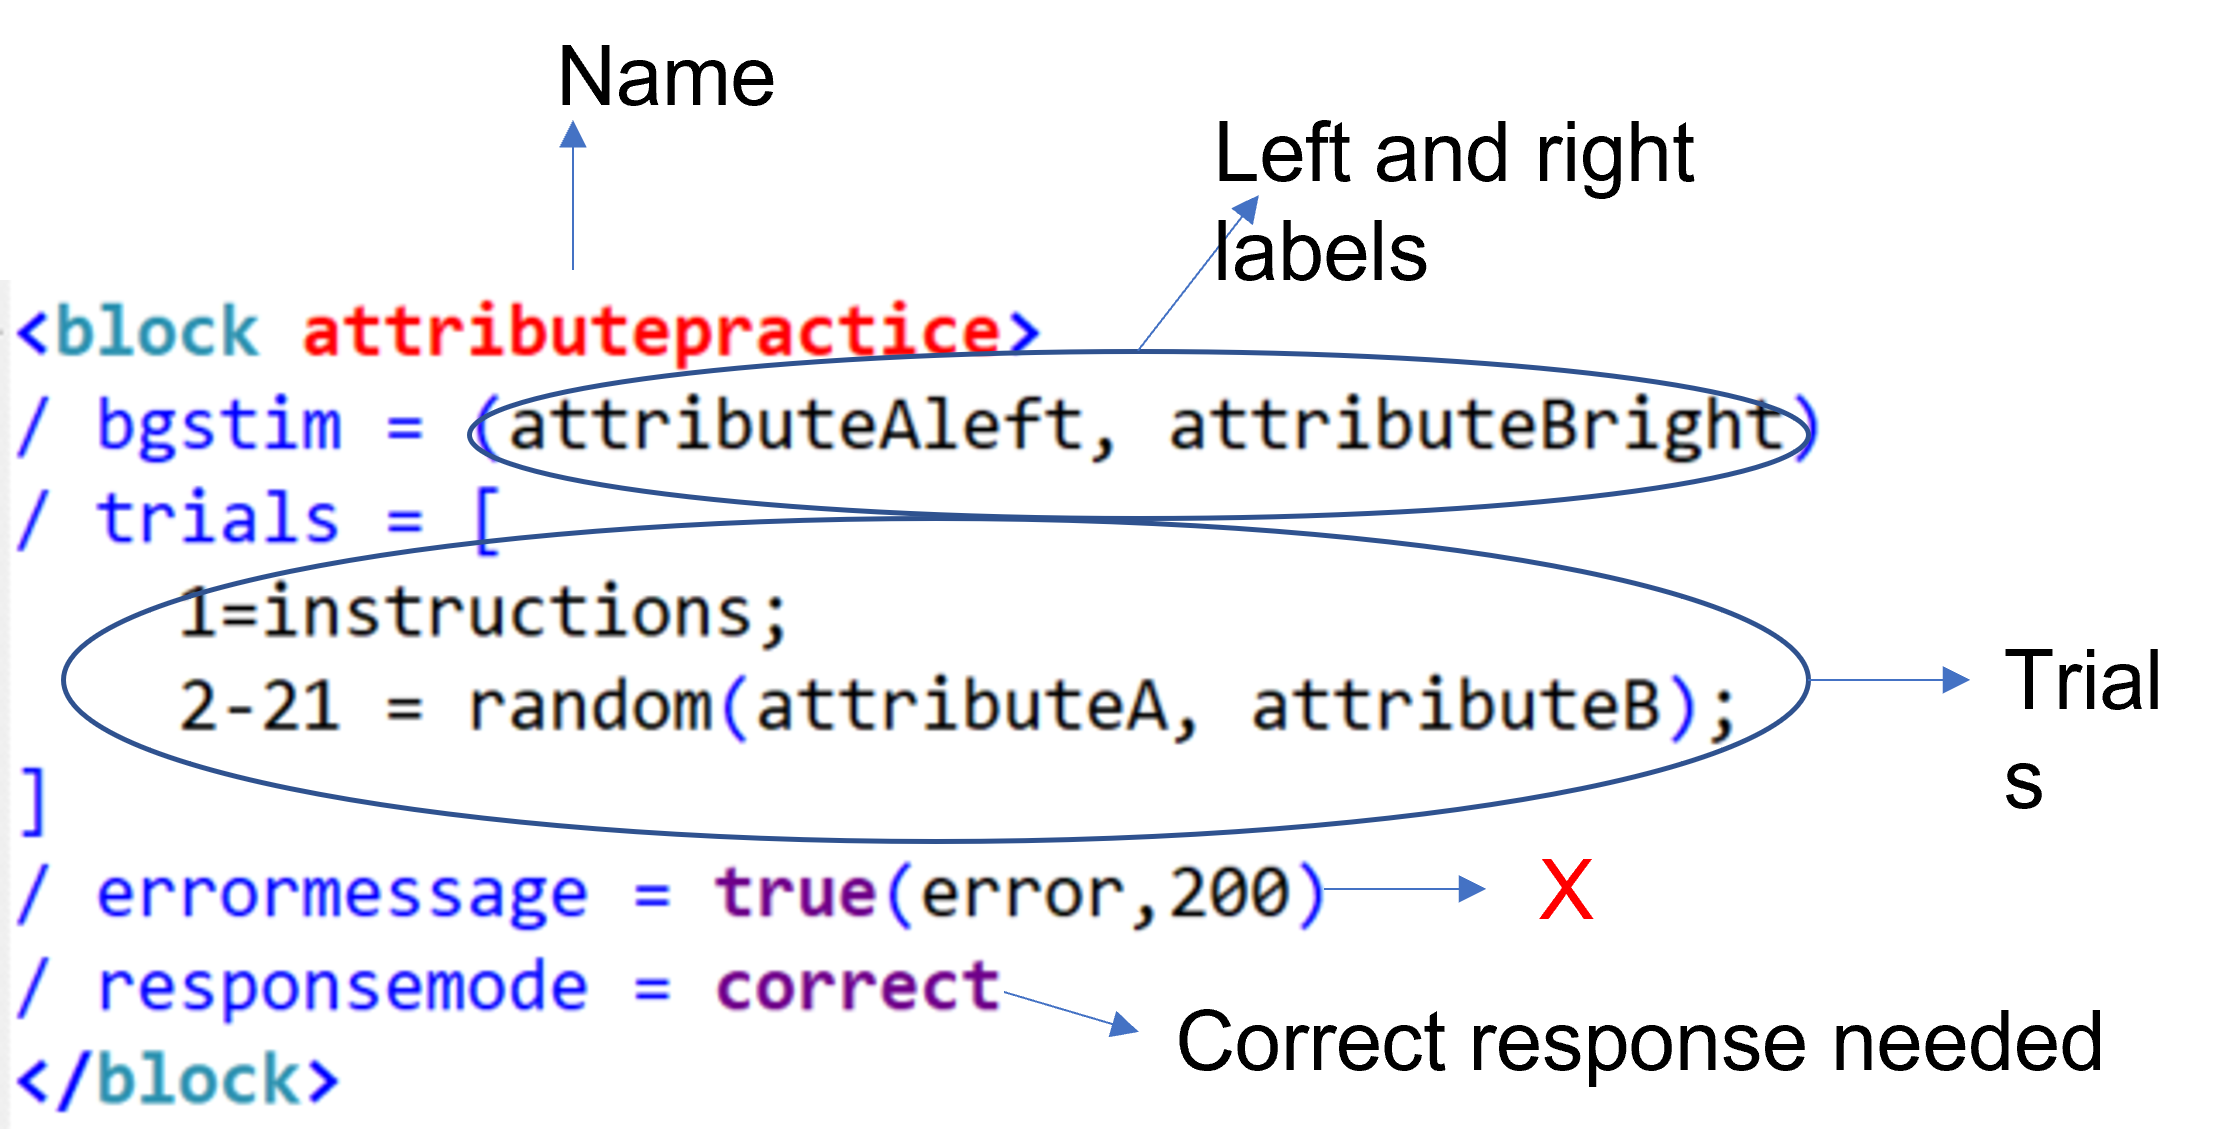
\includegraphics[width=.80\linewidth]{block.png}
%	\end{figure}
Il primo trial è un trial di istruzioni. 

I trial da 2 a 21 sono trial sperimentali in cui vengono presentati (a caso) gli stimoli definiti in \texttt{attributeA} e \texttt{attributeB}

Totale trial effettivi = 20
	\end{small}
\end{frame}

\begin{frame}[fragile]
	Per i blocchi di pratica pura degli stimoli target, si deve fare attenzione al posizionamento delle etichette sulla base della condizione che segue (compatibile/incompatibile): 
	
	\vspace{3mm}
\begin{columns}
	\begin{column}{.50\linewidth}
	\begin{small}
		Pratica compatibile:
		\begin{Verbatim}[commandchars=\\\{\}]
<block \textcolor{red}{targetcompatiblepractice}>
/ bgstim = (\textcolor{red}{targetAleft}, 
\textcolor{red}{targetBright})
/ trials = [
1=instructions;
2-21 = random(\textcolor{blue}{targetAleft},
 \textcolor{blue}{targetBright});
]
/ errormessage = true(error,200)
/ responsemode = correct
</block>
		\end{Verbatim}
	\end{small}
	\end{column}
\begin{column}{.50\linewidth}
	\begin{small}
		Pratica incompatibile:
		\begin{Verbatim}[commandchars=\\\{\}]
<block \textcolor{red}{targetincompatiblepractice}>
/ bgstim = (\textcolor{red}{targetAright}, 
\textcolor{red}{targetBleft})
/ trials = [
1=instructions;
2-21 = random(\textcolor{blue}{targetAright},
 \textcolor{blue}{targetBleft});
]
/ errormessage = true(error,200)
/ responsemode = correct
</block>
		\end{Verbatim}
	\end{small}
\end{column}
\end{columns}
\end{frame}


\begin{frame}[fragile]{Blocchi associativi di pratica}
	\begin{small}
		\begin{Verbatim}[commandchars=\\\{\}]
<block \textcolor{red}{compatibletest1}>
/ bgstim = (\textcolor{red}{targetAleftmixed, orleft,  attributeAleft,}
\textcolor{red}{targetBrightmixed, orright, attributeBright})
/ trials = [
1=\textcolor{red}{instructions};
\textcolor{red}{3,5,7,9,11,13,15,17,19,21}= random(\textcolor{blue}{targetAleft}, \textcolor{blue}{targetBright});
\textcolor{red}{2,4,6,8,10,12,14,16,18,20} = random(\textcolor{blue}{attributeA}, \textcolor{blue}{attributeB})]
/ errormessage = true(error,200)
/ responsemode = correct
  [...]
</block>
		\end{Verbatim}
	\end{small}
Il primo trial è sempre un trial di istruzione\\ Gli stimoli immagine e attributo si alternano\\Totale trial effettivi = 20

\end{frame}

\begin{frame}[fragile]{Blocchi associativi di test}
	\begin{small}
		\begin{Verbatim}[commandchars=\\\{\}]
<block \textcolor{red}{compatibletest2}>
/ bgstim = (\textcolor{red}{targetAleftmixed, orleft,  attributeAleft,}
\textcolor{red}{targetBrightmixed, orright, attributeBright})
/ trials = [
\textcolor{red}{2,4,6,8,10,12,14,16,18,20,22},
\textcolor{red}{24,26,28,30,32,34,36,38,40} = random(targetAleft, targetBright);
\textcolor{red}{1,3,5,7,9,11,13,15,17,19,21,23},
\textcolor{red}{25,27,29,31,33,35,37,39} = random(attributeA, attributeB)]
/ errormessage = true(error,200)
/ responsemode = correct
[...]
</block>
		\end{Verbatim}
	\end{small}
 Gli stimoli immagine e attributo si alternano\\Totale trial = 40
	
\end{frame}

\begin{frame}
	\begin{center}
		
\includegraphics[width=.20\linewidth]{work.png}
	\end{center}
	\begin{itemize}
				\item Diminuite il numero dei trial nei blocchi di pura pratica
		
		\item Aumentate il numero di trial nei blocchi di pratica associative
		
	\end{itemize}
\end{frame}

\subsection*{Summary e dati}

\begin{frame}{Summary dei risultati}
	\begin{figure}
		\centering
		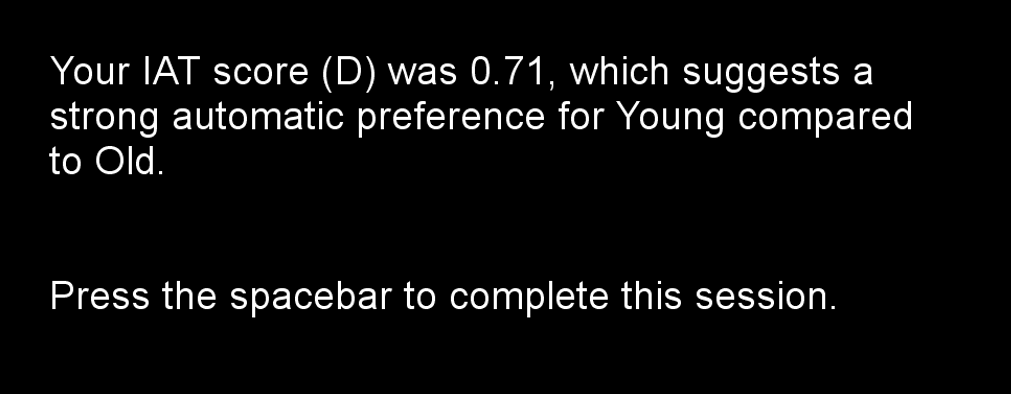
\includegraphics[width=\linewidth]{summary}
	\end{figure}
	
\end{frame}


\begin{frame}
	Si può dare una restituzione dei risultati immediata ai partecipanti (è il default di Inquisit)
	
	Lo script è già pronto per darvi una restituzione dei risultati, ossia per calcolare il \emph{D} score e farlo vedere ai partecipanti
	
	\begin{exampleblock}{Pros}
		è carino dare una restituzione immediata ai partecipanti 
		
		Potete salvare direttamente il \emph{D} score nel file \texttt{dat} $\rightarrow$ risultati e dati nello stesso file
	\end{exampleblock} 

\begin{alertblock}{Cons}
	Non dare la restituzione \textbf{prima} di un eventuale questionario
	
	Non si sa di preciso quale sia il \emph{D} score calcolato da Inquisit $\rightarrow$ problemi di replicabilità
\end{alertblock}
\end{frame}

\begin{frame}[fragile]
	Definire gli elementi che verranno usati per il summary:
	\begin{footnotesize}
		\begin{Verbatim}[commandchars=\\\{\}]
<trial summary>
/ ontrialbegin = [
values.magnitude = "little to no";
if( abs(expressions.d) > 0.15 ) values.magnitude = \textcolor{red}{"a slight";}
if( abs(expressions.d) > 0.35 ) values.magnitude = \textcolor{red}{"a moderate"};
if( abs(expressions.d) >= 0.65 ) values.magnitude = \textcolor{red}{"a strong"};
if (expressions.d >= 0.0) \textcolor{red}{values.preferred} = item.targetALabel.1;
if (expressions.d < 0.0) \textcolor{red}{values.preferred} = item.targetBLabel.1;
if (expressions.d < 0.0) \textcolor{red}{values.notpreferred}= item.targetALabel.1;
if (expressions.d >= 0.0) \textcolor{red}{values.notpreferred}= item.targetBLabel.1;
]
/ stimulustimes = [0=summary]
/ validresponse = (" ")
/ recorddata = false
</trial>
		\end{Verbatim}
	\end{footnotesize}	
\end{frame}

\begin{frame}[fragile]
	Definire il testo del summary: 
	\begin{footnotesize}
		\begin{Verbatim}[commandchars=\\\{\}]
<text summary>
/ items = ("Your IAT score (D) was \textcolor{red}{<% expressions.d %>}, 
	which suggests \textcolor{red}{<% values.magnitude %>} automatic preference 
	for \textcolor{red}{<% values.preferred %>} compared to \textcolor{red}{<% values.notpreferred %>}.
	~n~n~nPress the spacebar to complete this session.") 
/ size = (60%, 60%)
/ hjustify = left
</text>

		\end{Verbatim}
	\end{footnotesize}	

\end{frame}

\begin{frame}[fragile]
	Infine, definiamo il blocco: 
	\begin{small}
		\begin{Verbatim}[commandchars=\\\{\}]
<block summary>
\textcolor{blue}{/ skip = [parameters.showsummaryfeedback == false]}
/ trials = [1=summary]
/ recorddata = false
</block>
		\end{Verbatim}
	\end{small}
... con le dovute accortezze: 
\begin{small}
\begin{Verbatim}[commandchars=\\\{\}]
<parameters>
/showsummaryfeedback = true
/ISI = 250
</parameters>
\end{Verbatim}
\end{small}
\end{frame}


\begin{frame}{Da dove viene \texttt{expression.d}?}
	
\begin{figure}
	\centering
	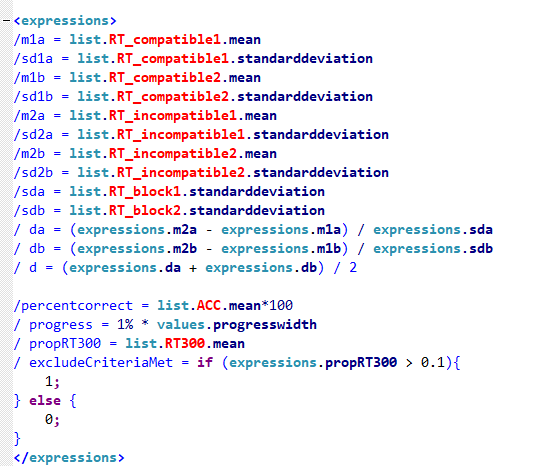
\includegraphics[width=0.7\linewidth]{expressions}
\end{figure}

\end{frame}


\begin{frame}[fragile]{Salvare i dati }
	\begin{small}
		\begin{Verbatim}[commandchars=\\\{\}]
<data>
/ columns = (\textcolor{red}{build, computer.platform, date, time,} \textcolor{template}{subject}, 
\textcolor{blue}{group, session}, \textcolor{template}{blockcode}, \textcolor{template}{blocknum}, 
\textcolor{template}{trialcode, trialnum, values.conditionOrder,}
\textcolor{template}{response, correct, latency}, 
\textcolor{template}{stimulusnumber, stimulusitem}, 
\textcolor{blue}{expressions.da, expressions.db, expressions.d}, 
\textcolor{blue}{	expressions.percentcorrect,} 
\textcolor{blue}{expressions.propRT300, expressions.excludeCriteriaMet})
</data>			
		\end{Verbatim}
	\end{small}
Possiamo togliere tutte le cose che non ci interessano. In \textcolor{template}{verde} gli indispensabili, in \textcolor{blue}{blu} i facoltativi, in \textcolor{red}{rosso} i superflui.
\end{frame}




\section{Experiment time!}


\begin{frame}[fragile]{Primo gruppo}
	\begin{footnotesize}
			\begin{Verbatim}[commandchars=\\\{\}]
<expt>
/ onexptbegin = [
 values.conditionOrder = "c-ic" %ordine condizioni associative
 ]
/ preinstructions = (iatintro) % Pagina di benvenuto
\textcolor{blue}{/ groups = (1 of 2)} % Definizione ordine presentazione
/ blocks = [   % L'esperimento vero e proprio
1=targetcompatiblepractice; 2=attributepractice; 
3=compatibletest1; 4=compatibletestinstructions;	
5=compatibletest2; 
6=targetincompatiblepractice; 7=incompatibletest1; 
8=incompatibletestinstructions; 9=incompatibletest2; 
10=summary;  % pagina del d score
11 = end; % grazie e arrividerci
			]
</expt>
		\end{Verbatim}
	\end{footnotesize}
\end{frame}


\begin{frame}[fragile]{Secondo gruppo}
	\begin{footnotesize}
		\begin{Verbatim}[commandchars=\\\{\}]
<expt>
/ onexptbegin = [
values.conditionOrder = "ic-c"
]
/ preinstructions = (iatintro)
\textcolor{blue}{/ groups = (2 of 2)} % cambia l'assegnazione di gruppo
/ blocks = [ 
1=targetincompatiblepractice; 	2=attributepractice; 
3=incompatibletest1; 4=incompatibletestinstructions; 
5=incompatibletest2; 
6=targetcompatiblepractice; 7=compatibletest1; 
8=compatibletestinstructions; 9=compatibletest2; 
10=summary;
11 = end;
			]
</expt>
		\end{Verbatim}
	\end{footnotesize}
\end{frame}

\begin{frame}
	Si possono avere tutti i gruppi che si vogliono, a seconda del numero di condizioni sperimentali 
	
	In questo caso: 
	
	\begin{itemize}
		\item Tutti i soggetti assegnati al gruppo 1 \texttt{/ groups = (1 of 2)} vedono prima la condizione compatibile e poi quella incompatibile
			\item Tutti i soggetti assegnati al gruppo 2 \texttt{/ groups = (2 of 2)} vedono prima la condizione incompatibile e poi quella compatibile
	\end{itemize}

Se avessimo un questionario, dovremmo specificare qui l'ordine in cui vogliamo presentarlo rispetto alle misure implicite
\end{frame}

\section{Tempo di modifiche}

\begin{frame}
	La prima cosa da fare, ovviamente, è tradurre il tutto in italiano (vi lascio divertire)
	
	\vspace{5mm}
	Attenzione! Per non complicare troppo le operazioni, si possono tradurre solo le parti che i partecipanti vedranno
	 
\end{frame}

\begin{frame}
	Togliamo questo: 
	
	\begin{figure}
		\centering
		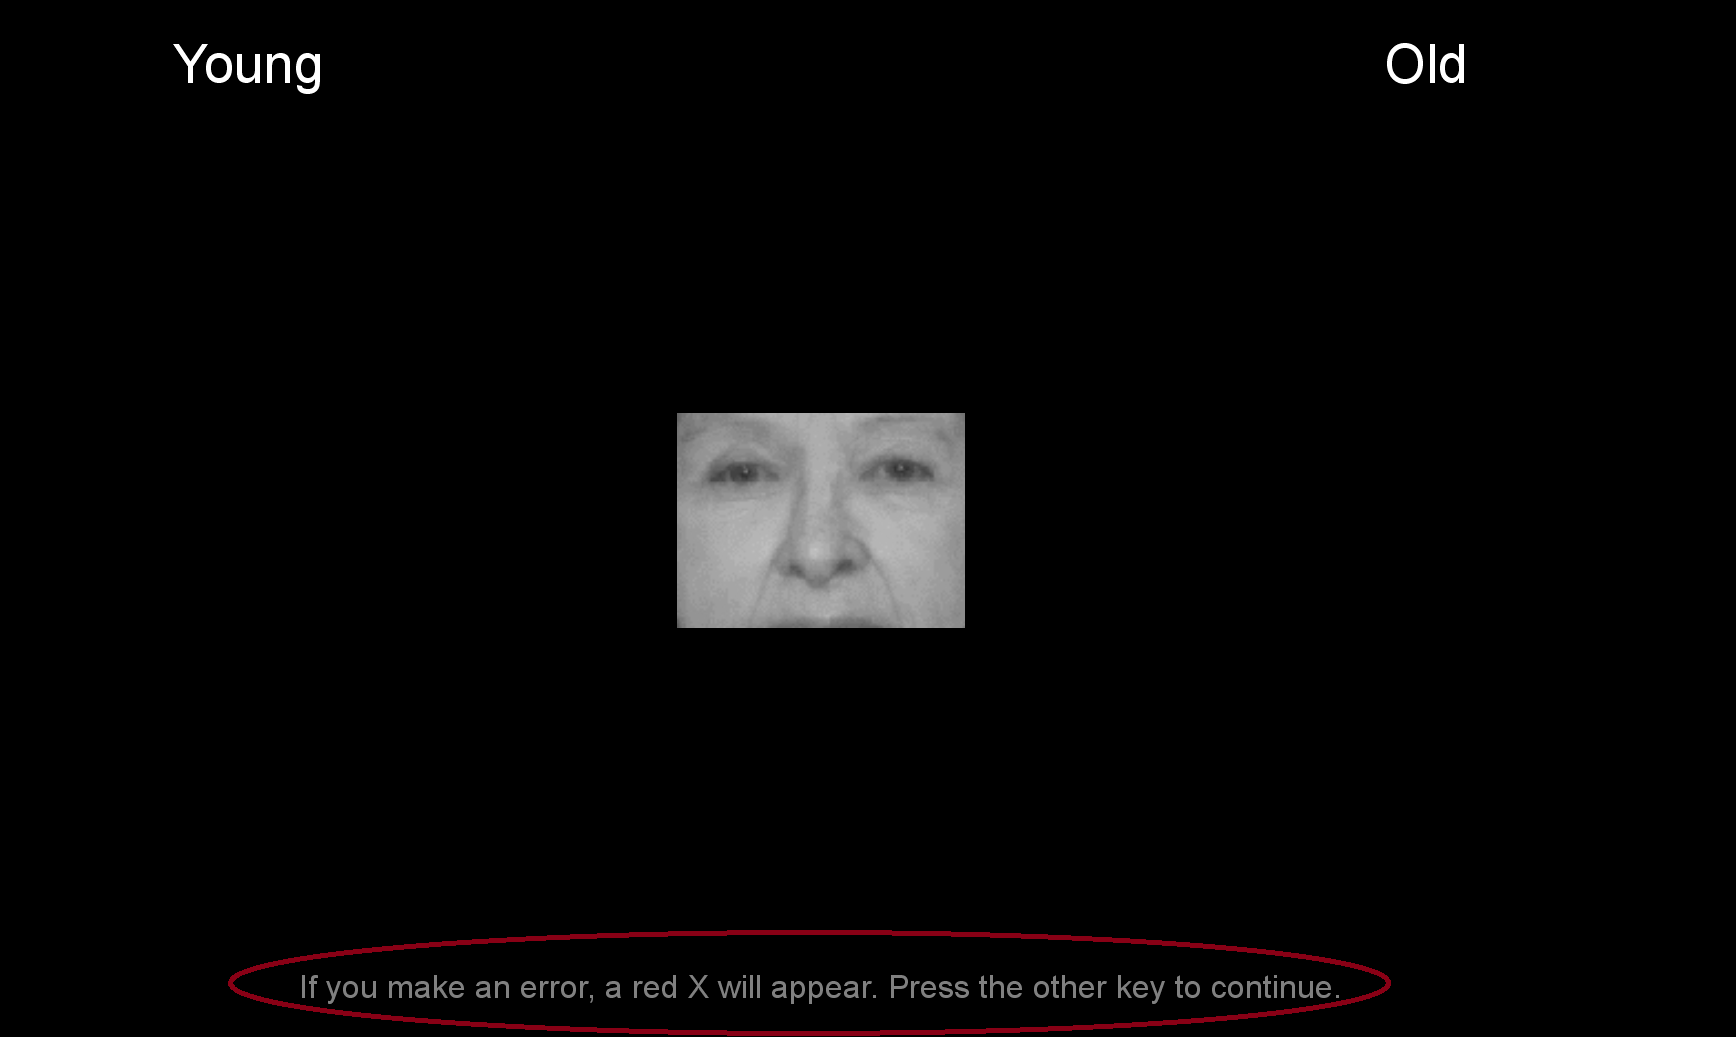
\includegraphics[width=.70\linewidth]{remind.png}
	\end{figure}

Perché: 

\begin{itemize}
	\item Il partecipante rimane troppo esposto allo stimolo
	\item Il tempo di risposta è falsato
	\item Durante l'esperimento può essere distraente
\end{itemize}

\end{frame}


\begin{frame}[fragile]
	Step 1: Identificare come si chiama l'elemento: 
	\begin{small}
		\begin{Verbatim}[commandchars=\\\{\}]
<trial attributeA>
/ validresponse = ("E", "I")
/ correctresponse = ("E")
/ stimulusframes = [1 = attributeA, \textcolor{red}{errorReminder}] %eccolo! 
/ posttrialpause = parameters.ISI
</trial>
	\end{Verbatim}
	\end{small}

Va tolto da tutti i trial nel file: 
	\begin{small}
				\begin{verbatim}
				<trial attributeA>
				[...]
				/ stimulusframes = [1 = attributeA] 
				[...]
				</trial>
				
			\end{verbatim}
		\end{small}
	
\end{frame}


\begin{frame}[fragile]{Reminder}
		Ora però l'esperimento inizia brutalmente subito dopo la pagina di istruzioni, per cui il tempo di risposta del primo trial di ogni blocco potrebbe non essere attendibile. 
		
		Mettiamo una pagina che permetta al partecipante di capire cosa sta per succedere e di prepararsi: 


\begin{figure}
	\centering
	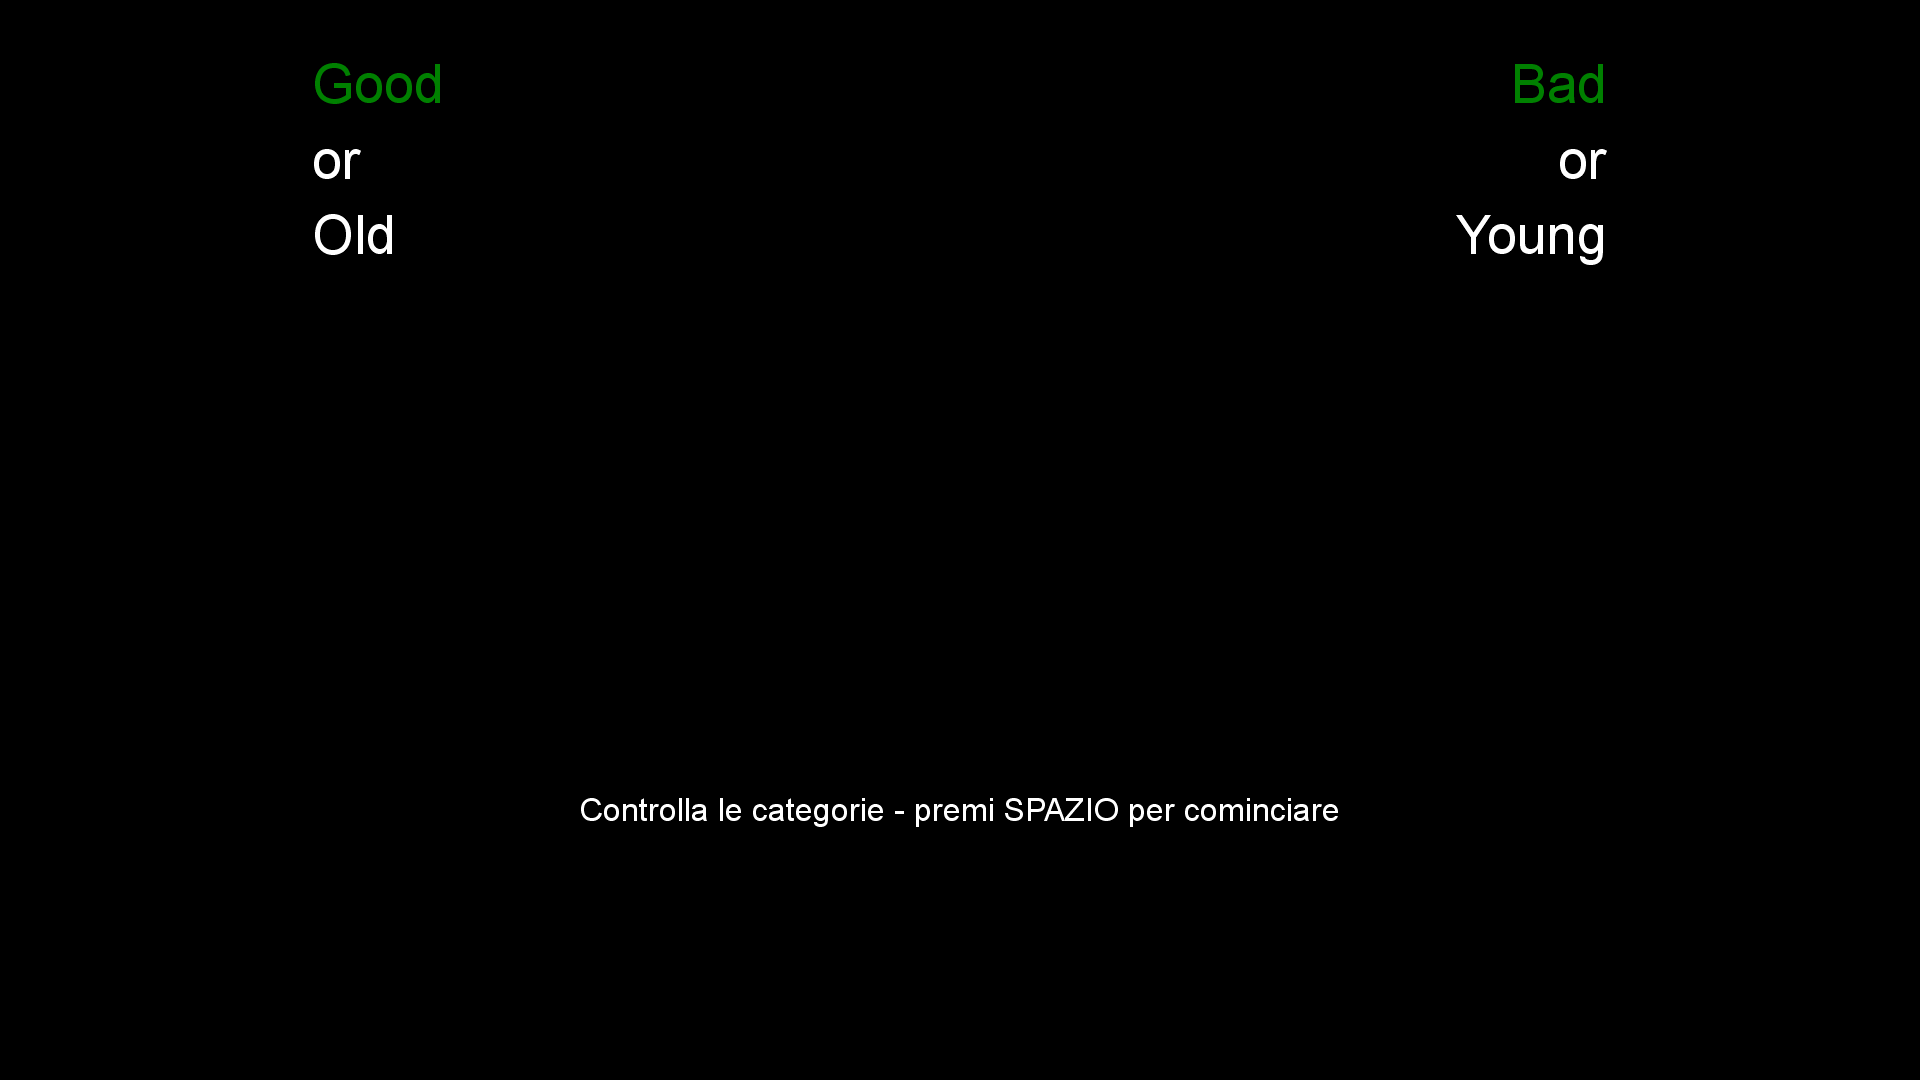
\includegraphics[width=0.7\linewidth]{trial}
\end{figure}


	
\end{frame}

\begin{frame}[fragile]
	Definiamo l'oggetto e il suo aspetto tutto insieme:
		\begin{small}
\begin{Verbatim}[commandchars=\\\{\}]
<text reminder>
\textcolor{red}{/ items = ("Controlla le categorie - premi }
	\textcolor{red}{SPAZIO per cominciare")}
/ position = (50%, 75%) 
/ color = (255, 255, 255)
/ fontstyle = ("Arial", 3%, false, false, false, false, 5, 1)
</text>
\end{Verbatim}
	\end{small}

Definiamo il suo comportamento:
	\begin{small}
		\begin{verbatim}
			<trial reminder> 
			/ correctresponse = (" ") 
			/ frames = [1=reminder] 
			/ responsemode = correct 
			</trial>
		\end{verbatim}
	\end{small}
\end{frame}

\begin{frame}[fragile]

\begin{Verbatim}[commandchars=\\\{\}]
<block attributepractice>
/ bgstim = (attributeAleft, attributeBright)
/ trials = [
1=instructions;
\textcolor{red}{2=reminder;} %va aggiunto nella definizione del blocco
3-22 = random(attributeA, attributeB);
]
/ errormessage = true(error,200)
/ responsemode = correct
</block>
	\end{Verbatim}
Attenzione a modificare il numero di trial!!

Questa operazione va fatta per tutti i blocchi che si vogliono modificare
\end{frame}

\begin{frame}[fragile]{Togliere ``or''}
	Bisogna andare nella definizione dei blocchi dello IAT: 
	\begin{small}
		\begin{Verbatim}[commandchars=\\\{\}]
<block compatibletest1>
/ bgstim = (targetAleftmixed, \textcolor{red}{orleft}, attributeAleft,
 targetBrightmixed, \textcolor{red}{orright}, attributeBright)
/ trials = [
1=reminder;
3,5,7,9,11,13,15,17,19,21= random(targetAleft, targetBright);
2,4,6,8,10,12,14,16,18,20 = random(attributeA, attributeB)]
/ errormessage = true(error,200)
/ responsemode = correct
[...]
</block>
		\end{Verbatim}
	\end{small}
\end{frame}

\begin{frame}
	Se però non si modifica la posizione di \texttt{targetAleftmixed} e  \texttt{targetBleftmixed}, il risultato non è molto carino: 
	
	\begin{figure}
		\centering
		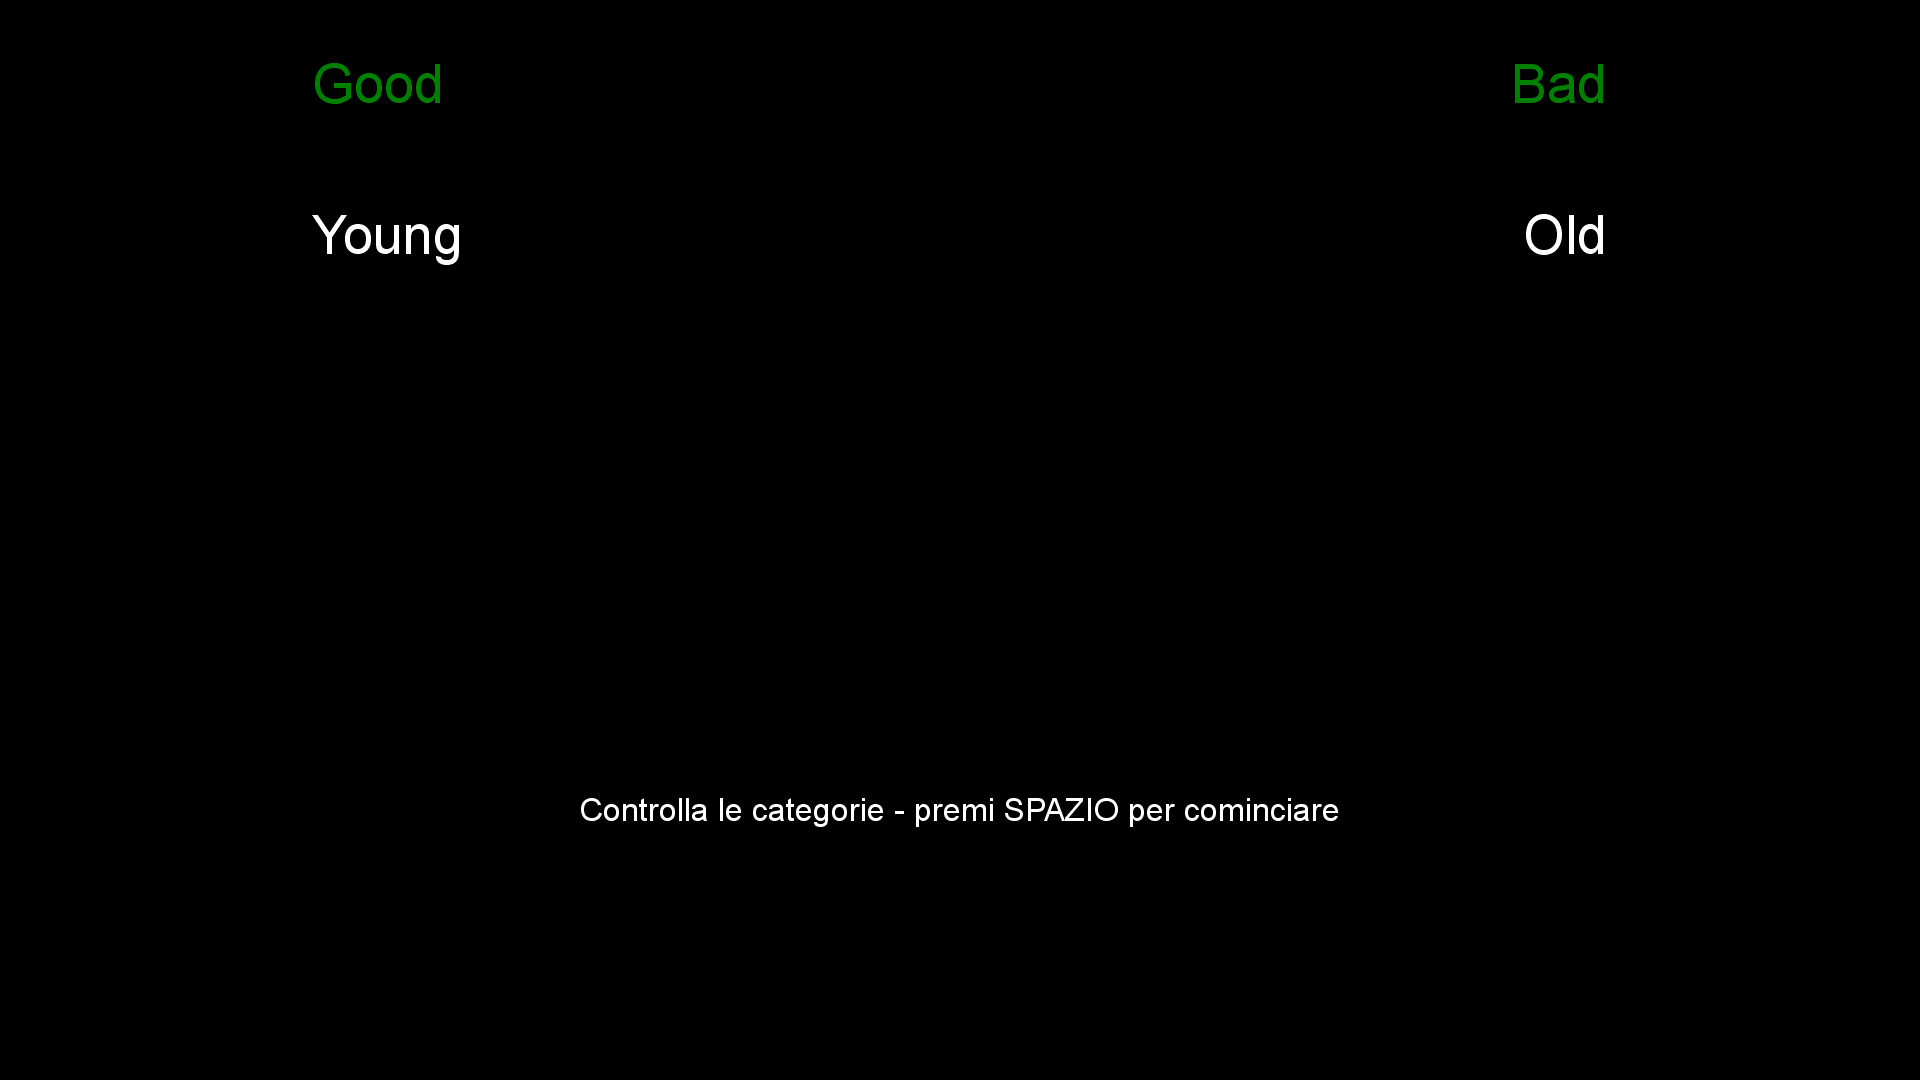
\includegraphics[width=0.7\linewidth]{trialBrutto}
	\end{figure}
\end{frame}

\begin{frame}[fragile]
	\begin{small}
		\begin{Verbatim}[commandchars=\\\{\}]
<text targetBleftmixed>
/ items = targetBlabel
/ valign = top
/ halign = left
/ position = (5%, \textcolor{red}{19%}) % cambiato in 10%
/ fontstyle = ("Arial", 5%)
</text>
\end{Verbatim}
\end{small}

\begin{figure}
	\centering
	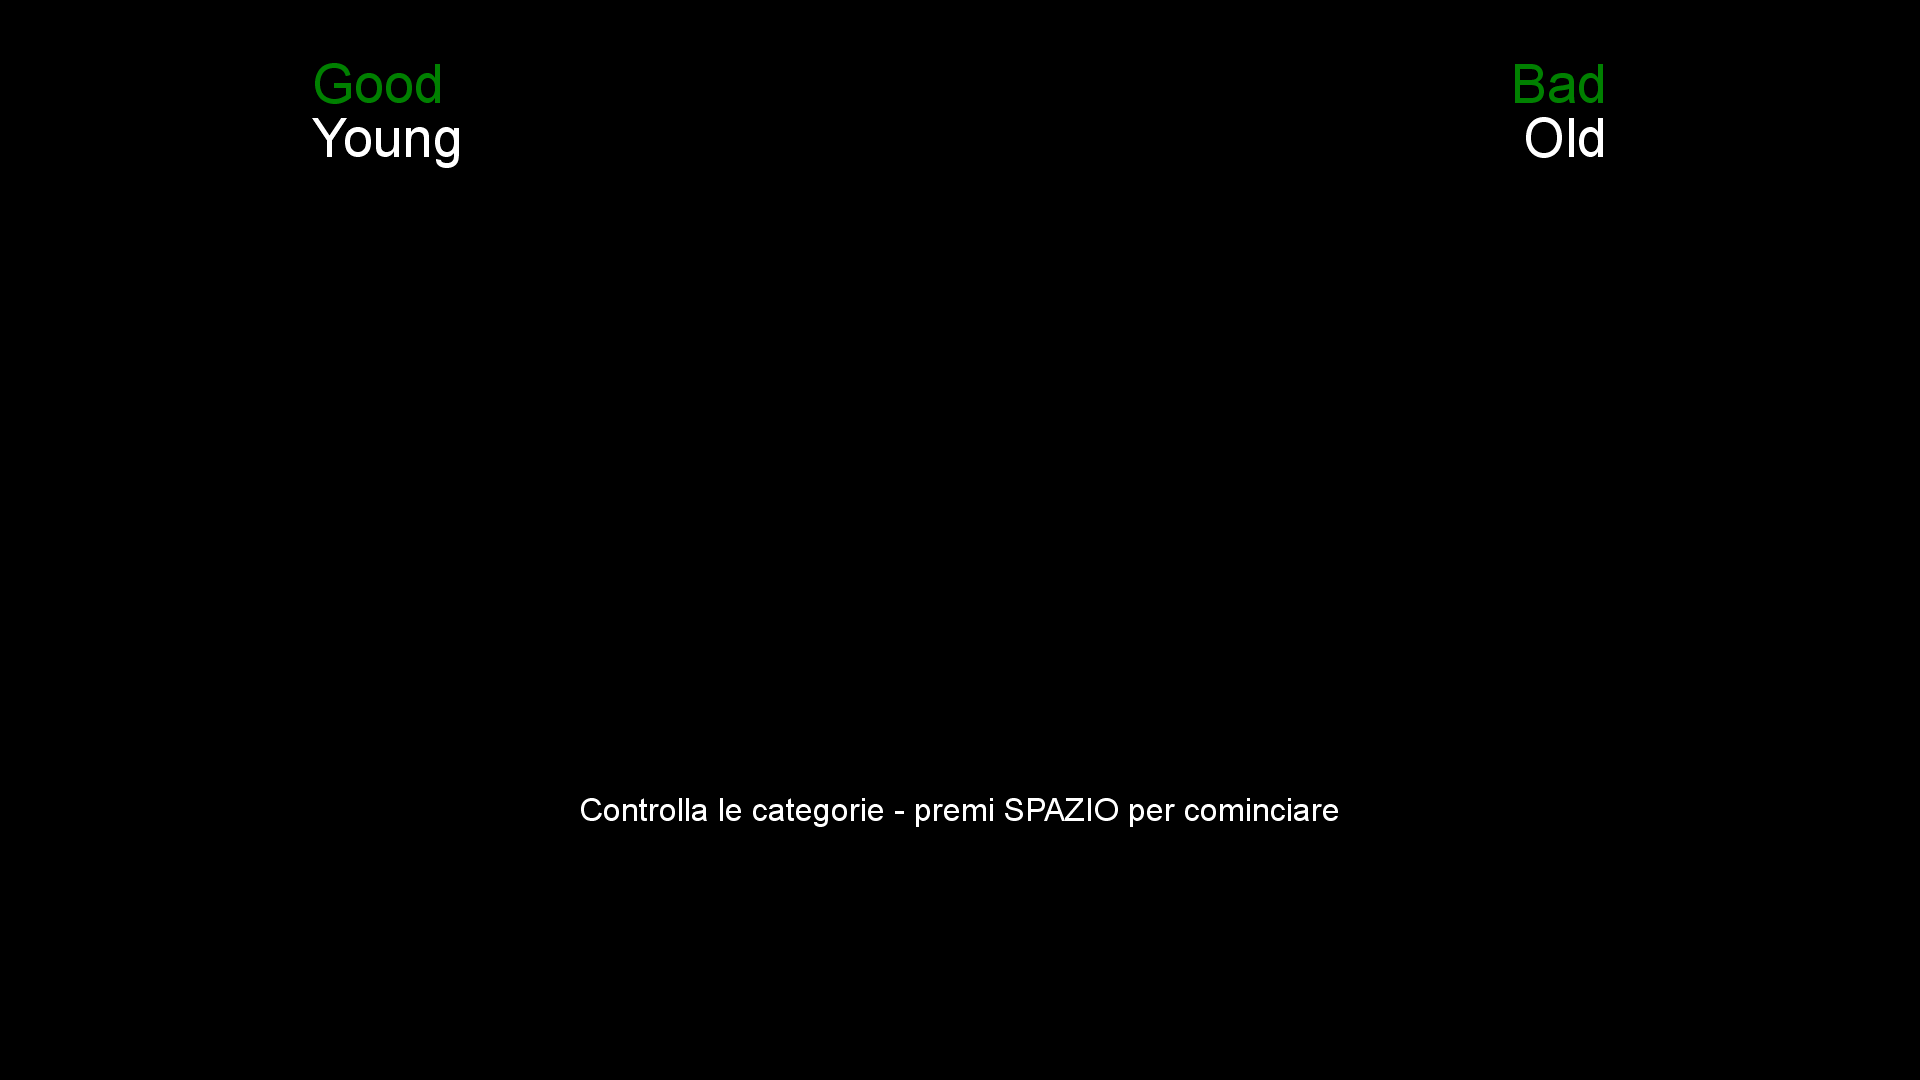
\includegraphics[width=0.5\linewidth]{trialBello}
\end{figure}

\end{frame}

\begin{frame}
	\begin{center}
		
\includegraphics[width=.20\linewidth]{work.png}
	\end{center}
	\begin{itemize}
		\item Aggiungere il trial reminder
		
		\item Togliere \texttt{or} dalla slide e avvicinare le etichette
		
	\end{itemize}
\end{frame}

\subsection*{Domande esplicite}

\begin{frame}{Domande esplicite}
	A \href{https://www.millisecond.com/support/docs/current/html/language/languagereference.htm}{\textcolor{blue}{questo indirizzo}}, sotto la voce ``Surveys'' vengono riportate le varie opzioni per creare domande esplicite 
	
	Quelle più usate sono: 
	
	\begin{itemize}
	 \item \texttt{checkboxes}: Permettono di scegliere più di un'opzione
	 \item  \texttt{dropdown}: Permette di scegliere un'opzione dal menu a tendina
	 \item \texttt{radiobuttons}: Permette di scegliere un'opzione tra una serie di opzioni
	 \item \texttt{slider}: Permette di indicare il grado di accordo verso due estremi
	\end{itemize}

Se ne possono creare di diverse e mettere tutte nella stessa pagina 
\end{frame}

\begin{frame}
	Creiamo una scheda socio-demografica dove chiediamo: 
	
	\begin{itemize}
		\item Sesso
		\item Età 
		\item Occupazione
	\end{itemize}

Creiamo un piccolo questionario dove chiediamo: 
\begin{itemize}
	\item Grado di accordo con l'affermazione: ``Le persone giovani mi stanno simpatiche''
	\item Grado di accordo con l'affermazione: ``Le persone anziane mi stanno simpatiche''
\end{itemize}

Scheda e questionario andranno su due pagine diverse
\end{frame}

\begin{frame}[fragile]{Genere}
	
	Usiamo \texttt{radiobuttons}: 
	
	\begin{Verbatim}[commandchars=\\\{\}]
<radiobuttons \textcolor{blue}{genere}>
/ caption = "Genere"
/ options = ("Femmina", "Maschio", "Altro")
/orientation = horizontal, 
/fontstyle = ("Arial", 22)
/responsefontstyle = ("Arial",20)
</radiobuttons>
	\end{Verbatim}
	
\end{frame}

\begin{frame}[fragile]{Età}
	Usiamo \texttt{dropdown}:
	\begin{small}
\begin{Verbatim}[commandchars=\\\{\}]
<dropdown \textcolor{blue}{età}>
/ caption = "Età in anni compiuti"
/fontstyle = ("Arial", 22)
/ responsefontstyle = ("Arial", 20)
/ options = ("17", "18", "19", "20", ... , "più di 45")
/ optionvalues = ("17", "18", "19", "20", ... , "più di 45")
</dropdown>
\end{Verbatim}
	\end{small}

\end{frame}

\begin{frame}[fragile]{Occupazione}
\begin{Verbatim}[commandchars=\\\{\}]
<checkboxes \textcolor{blue}{occupazione}>
/caption = "Scegli la tua occupazione 
 (puoi indicare più di una risposta)''
/fontstyle = ("Arial", 22)
/ responsefontstyle = ("Arial", 20)
/options =  ("Lavoratore", "Studente", "Disoccupato", 
 "Dottorando", "Assegnista")
/optionvalues = ("lav", "stud", "dis", "dott", "ass")
</checkboxes>
\end{Verbatim}
\end{frame}

\begin{frame}[fragile]
	Creiamo la pagina:
	\begin{Verbatim}[commandchars=\\\{\}]
<surveypage \textcolor{blue}{demografica}>
/ questions = [1=\textcolor{red}{genere}; 2=\textcolor{red}{età}; 3=\textcolor{red}{occupazione}] 
/ txcolor = black
/ finishlabel = "Pagina Successiva"
/ nextbuttonposition = (80,90)
/ showpagenumbers = false
/showquestionnumbers = false
</surveypage>
\end{Verbatim}

 e il relativo blocco che andrà poi messo in \texttt{<expt>}

\begin{Verbatim}[commandchars=\\\{\}]
 <block \textcolor{blue}{demografica}>
 /trials = [1=\textcolor{red}{demografica}]
 /screencolor =(170, 170, 170)
 </block>
\end{Verbatim}

\end{frame}

\begin{frame}[fragile]{La simpatia}
	\begin{footnotesize}
\begin{Verbatim}[commandchars=\\\{\}]
<slider \textcolor{blue}{giovani}>
/ caption = "Le persone giovani mi stanno simpatiche"
/ labels = ("1~nCompletamente in disaccordo", "2", "3",
 "4~nCompletamente d'accordo")
/ range = (1, 4)
/ defaultresponse = "1"
/increment = 0.5
/ position = (5%, 40%)
/ showticks = true
/ slidersize =(70%, 10%)
/ txcolor = black
/fontstyle = ("Arial", 20)
/responsefontstyle = ("Arial",16)
</slider>
\end{Verbatim}
	Ovviamente facciamo la stessa cosa per gli anziani cambiando l'etichetta \textcolor{blue}{giovani}
	\end{footnotesize}

\end{frame}

\begin{frame}[fragile]
	Creiamo la pagina:
\begin{Verbatim}[commandchars=\\\{\}]
<surveypage \textcolor{blue}{simpatia}>
/ questions = [1=\textcolor{blue}{giovani}; 2=\textcolor{blue}{anziani}] 
/ txcolor = black
/ finishlabel = "Pagina Successiva"
/ nextbuttonposition = (80,90)
/ showpagenumbers = false
/showquestionnumbers = false
</surveypage>
	\end{Verbatim}
E il relativo blocco  che andrà poi messo in \texttt{<expt>}: 
\begin{Verbatim}[commandchars=\\\{\}]
<block \textcolor{blue}{simpatia}>
/trials = [1=\textcolor{red}{simpatia}]
/screencolor =(170, 170, 170)
</block>
\end{Verbatim}
\end{frame}

\begin{frame}
	\begin{center}
		
\includegraphics[width=.20\linewidth]{work.png}
	\end{center}
	\begin{itemize}
		\item Creare la \texttt{surveypage} di demografica che contenga: 
		\begin{itemize}
			\item Età
			\item Genere
			\item Titolo di studio
		\end{itemize}
		
		
		\item Creare la \texttt{surveypage} di domande esplicite che contenga: 
		\begin{itemize}
			\item Simpatia per i giovani 
			\item Simpatia per gli anziani
		\end{itemize}
		
		\item Creare i rispettivi blocchi
	\end{itemize}
\end{frame}

\begin{frame}
	A questo punto abbiamo tutto e non dobbiamo far altro che metterlo in \texttt{<expt>}. Tuttavia: 
	
	\begin{itemize}
		\item Posizione fissa?
		\item Posizione alternata? (compito a casa!)
	\end{itemize}

In entrambi i casi, vanno modificate le istruzioni per introdurre al partecipante il fatto che l'esperimento non è ancora finito. 
\end{frame}


\begin{frame}[fragile]
Bisogna ``distruggere'' e creare le istruzioni: 
\begin{small}
\begin{Verbatim}[commandchars=\\\{\}]
<item \textcolor{blue}{IAT1}>
/1 = 
"In questa prova [...]"
</item>
\end{Verbatim}
Il loro aspetto:
\begin{Verbatim}[commandchars=\\\{\}]
<text \textcolor{blue}{IAT1}>
/ items = \textcolor{red}{IAT1}
/ hjustify = left
/ size = (90%, 60%)
/ position = (50%, 75%)
/ valign = bottom
/ select = sequence
/ txcolor = (255, 255, 255)
</text>
\end{Verbatim}
\end{small}

\end{frame}

\begin{frame}[fragile]
Il loro comportamento:
	\begin{small}
\begin{Verbatim}[commandchars=\\\{\}]
<trial \textcolor{blue}{IAT1}>
/ ontrialbegin = [
 values.progresswidth += 10;
 values.instructionIndex += 1;
]
/ stimulustimes = [1=\textcolor{red}{IAT1}, spacebar, 
 progressbar, progressbar_fill]
/ correctresponse = (" ")
/ errormessage = false
/ correctmessage = false
/ recorddata = false
</trial>
		\end{Verbatim}
	\end{small}
\end{frame}

\begin{frame}[fragile]
Il blocco da inserire nell'esperimento
	\begin{small}
\begin{Verbatim}[commandchars=\\\{\}]
<block \textcolor{blue}{IAT1}>
/trials = [1= \textcolor{red}{IAT1}]
/ recorddata = false
/responsemode = correct
</block>
		\end{Verbatim}
	\end{small}
\end{frame}

\begin{frame}
	Bisogna scrivere le istruzioni per ogni blocco dello IAT con il procedimento illustrato
	
	
	\vspace{3mm}
	\href{https://drive.google.com/file/d/11qOVR5-yGDc1lRPUpTt7327o9Z2Tt4_A/view?usp=sharing}{\textcolor{blue}{Qui}} trovate delle istruzioni che vi ho già preparato io 
	
	\vspace{3mm}
	Cosa manca? Le istruzioni per la scheda sociodemografica e le domande esplicite! 
\end{frame}

\begin{frame}[fragile]
	\begin{small}
			Le istruzioni:

\begin{Verbatim}[commandchars=\\\{\}]
<item \textcolor{blue}{demo_istruzioni}>
/1 = 
 "Per favore, compila il questionario che 
 apparirà nelle pagine seguenti"
</item>
\end{Verbatim}
		
		Il loro trial: 
		
		
		\begin{Verbatim}[commandchars=\\\{\}]
<trial \textcolor{blue}{demo_istruzioni}>
/ ontrialbegin = [
 values.progresswidth += 10;
 values.instructionIndex += 1;
]
/ stimulustimes = [1=\textcolor{red}{demo_istruzioni}, spacebar, 
 progressbar, progressbar_fill]
 [....]
</trial>
		\end{Verbatim}
	\end{small}
\end{frame}

\begin{frame}[fragile]
	 E infine il blocco:
		\begin{Verbatim}[commandchars=\\\{\}]
<block \textcolor{blue}{demo_istruzioni}>
/trials = [1= \textcolor{red}{demo_istruzioni}]
/ recorddata = false
/responsemode = correct
</block>
	\end{Verbatim}
\end{frame}

\subsection*{Posizione fissa}

\begin{frame}
	Bisogna impostare l'esperimento in \texttt{<expt>}
	
	Supponendo di volere mantenere la \textbf{posizione fissa in fondo}, non facciamo molta fatica: 
	
	\begin{itemize}
		\item Il numero di gruppi rimane invariato \textcolor{blue}{\texttt{/ group = (1 of 2)}}
		\item Bisogna aggiungere i nuovi blocchi in fondo (prima del summary e del grazie)
		\item  Tuttavia, vanno messe le nuove istruzioni! 
	\end{itemize}
\end{frame}

\begin{frame}[fragile]
	\begin{footnotesize}
		\begin{Verbatim}[commandchars=\\\{\}]
[....] %il resto rimane come prima
/ blocks = [
\textcolor{red}{1=IAT1;} 2=targetcompatiblepractice; 
\textcolor{red}{3=IAT2;} 3=attributepractice; 
\textcolor{red}{4=IAT3;} 4=compatibletest1; 
\textcolor{red}{5=IAT_pause;}
6=compatibletest2; 
\textcolor{red}{7=IAT4;}
8=targetincompatiblepractice; 
\textcolor{red}{9=IAT5;}
10=incompatibletest1; 
\textcolor{red}{11=IAT_pause;}
12=incompatibletest2; 
\textcolor{red}{13=demo_istruzioni;}
\textcolor{blue}{14=demografica;}
15=summary; 16=simpatia;
17 = end;
]
</expt>
		\end{Verbatim}
	\end{footnotesize}

\end{frame}

\begin{frame}[fragile]
	Se fate correre l'esperimento senza ulteriori modifiche $\rightarrow$ doppie istruzioni:

			\begin{footnotesize}
			\begin{Verbatim}[commandchars=\\\{\}]
<block attributepractice>
/ bgstim = (attributeAleft, attributeBright)
/ trials = [
	\textcolor{red}{1=instructions;}
	2-21 = random(attributeA, attributeB);
		]
/ errormessage = true(error,200)
/ responsemode = correct
</block>			
			\end{Verbatim}
			\end{footnotesize}
e si mette il reminder: 
			\begin{footnotesize}
			\begin{Verbatim}[commandchars=\\\{\}]
[...]
/ trials = [
\textcolor{red}{1=rerminder;}
2-21 = random(attributeA, attributeB);
]
[...]
			\end{Verbatim}
		\end{footnotesize}

\end{frame}

\begin{frame}[fragile]
	Questa operazione va fatta in tutti i blocchi dello IAT \underline{ad eccezione} dei blocchi associativi di test (quelli che sarebbero i blocchi 4 e 7): 
	
	\begin{footnotesize}
		\begin{Verbatim}[commandchars=\\\{\}]
<block compatibletest2>
/ bgstim = (targetAleftmixed, orleft, attributeAleft, targetBrightmixed, orright, attributeBright)
/ trials = [
 2,4,6,8,10,12,14,16,18,20,22,
 24,26,28,30,32,34,36,38,40 = random(targetAleft, targetBright);
 1,3,5,7,9,11,13,15,17,19,21,
 23,25,27,29,31,33,35,37,39 = random(attributeA, attributeB)]
 / errormessage = true(error,200)
 / responsemode = correct
[...]
</block>
	\end{Verbatim}
	\end{footnotesize}
Volendo si può inserire anche qui il reminder.... ma vanno ridefiniti tutti i trial!
\end{frame}

\subsection*{Posizione alternata}

\begin{frame}
	Bisogna lavorare di più e su più fronti ma il principio è lo stesso!
	
	I blocchi dello IAT rimangono invariati, ma cambia la loro posizione rispetto alla posizione della scheda socio demografica
	
	Ridefinire i gruppi di somministrazione sulla base della posizione della scheda socio demografica rispetto allo IAT
	

	\begin{tabular}{c  c  |c | c |}
		& \multicolumn{1}{c}{} & \multicolumn{2}{c}{Ordine scheda} \\
		& \multicolumn{1}{c}{} & \multicolumn{1}{c}{Prima} & \multicolumn{1}{c}{Dopo} \\
		\cline{3-4}
		\multirow{2}{*}{Ordine condizioni}& C - IC & Gruppo 1 &  Gruppo 2 \\
		\cline{3-4}
		& IC - C & Gruppo 3 & Gruppo 4 \\
		\cline{3-4} 
	\end{tabular}

\vspace{3mm}
\begin{small}
Soggetti Gruppo 1 $\rightarrow$ Scheda, IAT Compatibile - Incompatibile \\
Soggetti Gruppo 2 $\rightarrow$ IAT Compatibile-Incompatibile, scheda\\
Soggetti Gruppo 3  $\rightarrow$ Scheda, IAT Incompatibile - Compatibile \\
Soggetti Gruppo 4 $\rightarrow$ IAT  Incompatibile-Compatibile, scheda
\end{small}
\end{frame}

\begin{frame}[fragile]{Gruppo 1}
	Scheda, IAT C-IC:
	\begin{footnotesize}
		\begin{Verbatim}[commandchars=\\\{\}]
<expt>
/ onexptbegin = [
	values.conditionOrder = \textcolor{red}{"c-ic"}
	]
/ preinstructions = (iatintro)
\textcolor{red}{/ groups = (1 of 4)}
/ blocks = [
	\textcolor{blue}{1=demo_istruzioni;} \textcolor{blue}{2=demografica;} \textcolor{blue}{3=simpatia;}
	4=IAT1; 5=targetcompatiblepractice; 
	6=IAT2; 7=attributepractice; 
	8=IAT3; 9=compatibletest1; 
	10=IAT_pause; 11=compatibletest2; 
	12=IAT4; 13=targetincompatiblepractice; 
	14=IAT5;15=incompatibletest1; 
	16=IAT_pause; 17=incompatibletest2; 18=summary; 19= end;
			]
</expt>
			
		\end{Verbatim}
	\end{footnotesize}

\end{frame}


\begin{frame}[fragile]{Gruppo 2}
	IAT C-IC, Scheda:
	\begin{footnotesize}
		\begin{Verbatim}[commandchars=\\\{\}]
<expt>
/ onexptbegin = [
 values.conditionOrder = \textcolor{red}{"c-ic"}
 ]
/ preinstructions = (iatintro)
\textcolor{red}{/ groups = (2 of 4)}
/ blocks = [
	1=IAT1; 2=targetcompatiblepractice; 
	3=IAT2; 4=attributepractice;  
	5=IAT3; 6=compatibletest1; 
	7=IAT_pause; 8=compatibletest2; 
	9=IAT4; 10=targetincompatiblepractice; 
	11=IAT5;12=incompatibletest1; 
	13=IAT_pause; 14=incompatibletest2; 		
	\textcolor{blue}{15=demo_istruzioni;} 
	\textcolor{blue}{16=demografica;} \textcolor{blue}{17=simpatia;}
	18=summary; 19= end;
 ]
</expt>			
		\end{Verbatim}
	\end{footnotesize}
	
\end{frame}

\begin{frame}[fragile]{Gruppo 3}
	Scheda, IAT IC-C:
	\begin{footnotesize}
		\begin{Verbatim}[commandchars=\\\{\}]
<expt>
/ onexptbegin = [
 values.conditionOrder = \textcolor{red}{"ic-c"}
]
/ preinstructions = (iatintro)
\textcolor{red}{/ groups = (3 of 4)}
/ blocks = [
	\textcolor{blue}{1=demo_istruzioni;}  \textcolor{blue}{2=demografica;} \textcolor{blue}{3=simpatia;}
	4=IAT1; 5=targetincompatiblepractice; 
	6=IAT2; 7=attributepractice; 
	8=IAT3; 9=incompatibletest1; 
	10=IAT_pause; 11=incompatibletest2; 
	12=IAT4; 13=targetcompatiblepractice; 
	14=IAT5;15=compatibletest1; 
16=IAT_pause; 17=compatibletest2; 18=summary; 19= end;
]
</expt>
		\end{Verbatim}
	\end{footnotesize}
	
\end{frame}

\begin{frame}[fragile]{Gruppo 4}
 IC-C, Scheda
	\begin{footnotesize}
	\begin{Verbatim}[commandchars=\\\{\}]
<expt>
/ onexptbegin = [
values.conditionOrder = \textcolor{red}{"ic-c"}
]
/ preinstructions = (iatintro)
\textcolor{red}{/ groups = (4 of 4)}
/ blocks = [
	1=IAT1; 2=targetcompatiblepractice; 
	3=IAT2; 4=attributepractice; 
	5=IAT3; 6=compatibletest1; 
	7=IAT_pause; 8=compatibletest2; 
	9=IAT4; 10=targetincompatiblepractice; 
	11=IAT5;12=incompatibletest1; 
	13=IAT_pause; 14=incompatibletest2; 		
	\textcolor{blue}{15=demo_istruzioni;} 
	\textcolor{blue}{16=demografica;} \textcolor{blue}{17=simpatia;}
	18=summary; 19= end;
]
</expt>			
	\end{Verbatim}
\end{footnotesize}
	
\end{frame}
\section{A casa}

\begin{frame}
	Creare uno IAT per investigare quello che più vi interessa (e che ovviamente sia investigabile con lo IAT)
	
	\vspace{3mm}
	
	Aggiungere una scheda socio-demografica e di domande esplicite che includa almeno: 
	\begin{itemize}
		\item 4 domande di natura socio demografica (e.g., sesso, età, istruzione, educazione)
		\item  3 domande esplicite sullo stesso tema dello IAT (e.g., preferenza esplicita per una categoria, preferenza esplicita per la categoria opposta, preferenza comparativa tra le due categorie)
	\end{itemize}
\vspace{3mm}

 \href{https://drive.google.com/drive/folders/11J1KG9HegG8JcvxogtuJAfIhri_k7Xiy?usp=sharing}{\textcolor{blue}{In questa cartella}} trovate uno script di esempio di uno IAT per investigare la preferenza per il cioccolato 
\end{frame}

\end{document}